\documentclass[11pt,aps,preprint,nofootinbib,superscriptaddress,tightenlines]{revtex4-2}
\usepackage{amsmath,amssymb,bm,mathtools,graphicx}
\usepackage{xcolor}
\definecolor{darkblue}{RGB}{0,0,160}
\usepackage[colorlinks=true,linkcolor=darkblue,citecolor=darkblue,urlcolor=darkblue]{hyperref}

\def\st{\begin{equation}}
\def\stp{\end{equation}}
\def\Eq#1{eq.~(\ref{#1})}
\def\Sect#1{Sect.~\ref{#1}}
\def\Fig#1{Fig.~\ref{#1}}
\usepackage{dsfont}
\newcommand{\one}{\mathds{1}}
\newcommand{\avg}[1]{\langle #1\rangle}
\let\oldparagraph\paragraph
\renewcommand{\paragraph}{\par\bigskip\oldparagraph}

\begin{document}

\title{First full Hamiltonian stochastic runs}
\author{D.~Teaney}
\affiliation{Department of Physics and Astronomy, Stony Brook University,
Stony Brook, New York 11794, USA}
\date{\today}

\begin{abstract}
We couple the stochastic viscous step in the particle representation
(\texttt{stochrep.tex}) to the Hamiltonian (ideal SPH) step and run a uniform
two-dimensional fluid at rest, starting from zero momenta.  This note records
the setup and, for each test, what we found: the residual move is needed to
keep the lattice modes under control; with it, the fluid thermalizes and stays
stable, apart from a slow drift of the energies; the drift comes from the
stochastic step, not from the integrator, and the gradient-corrected change of
representation reduces it.
\end{abstract}

\maketitle

%=============================================================================
\section{Setup}
\label{sec:setup}

\paragraph{The time step.}  Each time step is that of \texttt{generic\_step!},
with the stochastic step in place of the deterministic viscous step:
\begin{enumerate}
\item a stochastic viscous half step, of length $\Delta t/2$;
\item the leapfrog (drift--kick--drift) of the ideal SPH Hamiltonian $H$, of
  length $\Delta t$;
\item a second stochastic half step.
\end{enumerate}
The stochastic step is \texttt{stochrep\_step!} of \texttt{stochrep.tex}: a
stress sweep and a residual sweep on a checkerboard of cells, at fixed
positions.  The order of the two sweeps alternates from step to step.  Before
each step the particle energies $e_a$ and volumes $V_a=s_a/S_a$ are recomputed from
the smoothed state, the coefficients are evaluated at the coarse-grained
velocity $\dot{\bm x}_a$, and after it the entropies are set by the back map.

\paragraph{Parameters.}
\begin{center}
\begin{tabular}{ll}
\hline
fluid & conformal, $c_s^2=1/3$, $\eta/s=0.2$, $\zeta=0$, three dimensions ($d=3$, $\zeta_{\rm eff}$) \\
box & periodic, $0.6\times0.589$ \\
lattice & hexagonal, $h=0.05$ \\
$h/a=2$ & $N=672$ particles, 56 bonds per star \\
$h/a=2.5$ & $N=1020$ particles, 88 bonds per star \\
entropy density & $S=10^6$: $T=90.9$, $s_a=541$ ($h/a=2$), $346$ ($h/a=2.5$) \\
thermal velocity & $\avg{\delta v^2}^{1/2}=0.043$ per component ($h/a=2$), $0.054$ ($h/a=2.5$) \\
time step & $\Delta t=8.66\times10^{-3}$, half the default viscous step \\
initial state & uniform, at rest, all momenta zero \\
\hline
\end{tabular}
\end{center}

\paragraph{Variants of the viscous step.}
\begin{itemize}
\item \emph{Stress and residual moves, $\lambda=1$}: detailed balance, every mode
  fluctuates.
\item \emph{Stress move and deterministic residual, $\lambda=\infty$}: the lattice
  modes are damped without noise and stay cold.
\item \emph{Stress move only.}
\end{itemize}
The vote is either per bond (the bond split of \texttt{stochrep.tex}) or a single
vote of the star.  The change of representation is either the plain exact map,
which holds $e_a$ fixed, or the gradient-corrected map of \texttt{changerep.tex},
which holds $e_a-g_a$ fixed and refits the gradient energy $g_a$ afterwards.

\paragraph{What is measured.}
\begin{itemize}
\item The kinetic energy, $\sum_a|\bm m_a|^2$, divided by its equilibrium value
  $2(N-1)V_awT$.
\item The momentum spectrum, $\avg{|\bm m_{\bm k}|^2}/(NV_awT)$, longitudinal and
  transverse, over the second half of the run.
\item The smoothed energy $H$, conserved by the leapfrog, and the sum of the
  particle energies $\sum_ae_a$, held fixed within a stochastic step.
\item The rms displacement of the particles from their initial sites, after
  removing the mean, and the \emph{local disorder}: the rms change of the
  distances between original nearest neighbours.  Both are in units of the
  lattice spacing $a$.  The first counts collective motion; the second does not.
\item The acceptance of the moves.
\end{itemize}
Scripts: \texttt{examples/stochrep\_hamiltonian.jl} and its plotting scripts.

%=============================================================================
\section{Is the residual move needed?}
\label{sec:needresid}

The stress move alone already satisfies detailed balance, so $e^{\mathbb S}$ is
stationary without the residual move.  The question is whether the residual
move is needed in practice.

\paragraph{What the stress move sees.}  With the stress move alone, a mode is
reached only through the fitted gradient.  It is damped, and receives noise, at
the resolved rate
\st
\Gamma_{\rm res}(k)=R(k)\,\Gamma(k),\qquad R(k)=\frac{K_{\rm res}(k)}{K(k)} ,
\stp
instead of the rate $\Gamma(k)$ of the bond form.  \Fig{fig:Rk}: the resolved
fraction $R$ depends only on $kh$, not on the lattice spacing, in 1D and 2D.  It
is close to one for $kh\ll1$, above $0.9$ for $kh\lesssim0.6$, equal to one half at
$kh\simeq1.6$, and negligible beyond $kh\simeq4$.  The zone edge is at $kh=\pi h/a$,
about $6$ for $h/a=2$.  Most lattice modes are therefore invisible to the stress
move, whatever the spacing.

\begin{figure}[t]
\centering
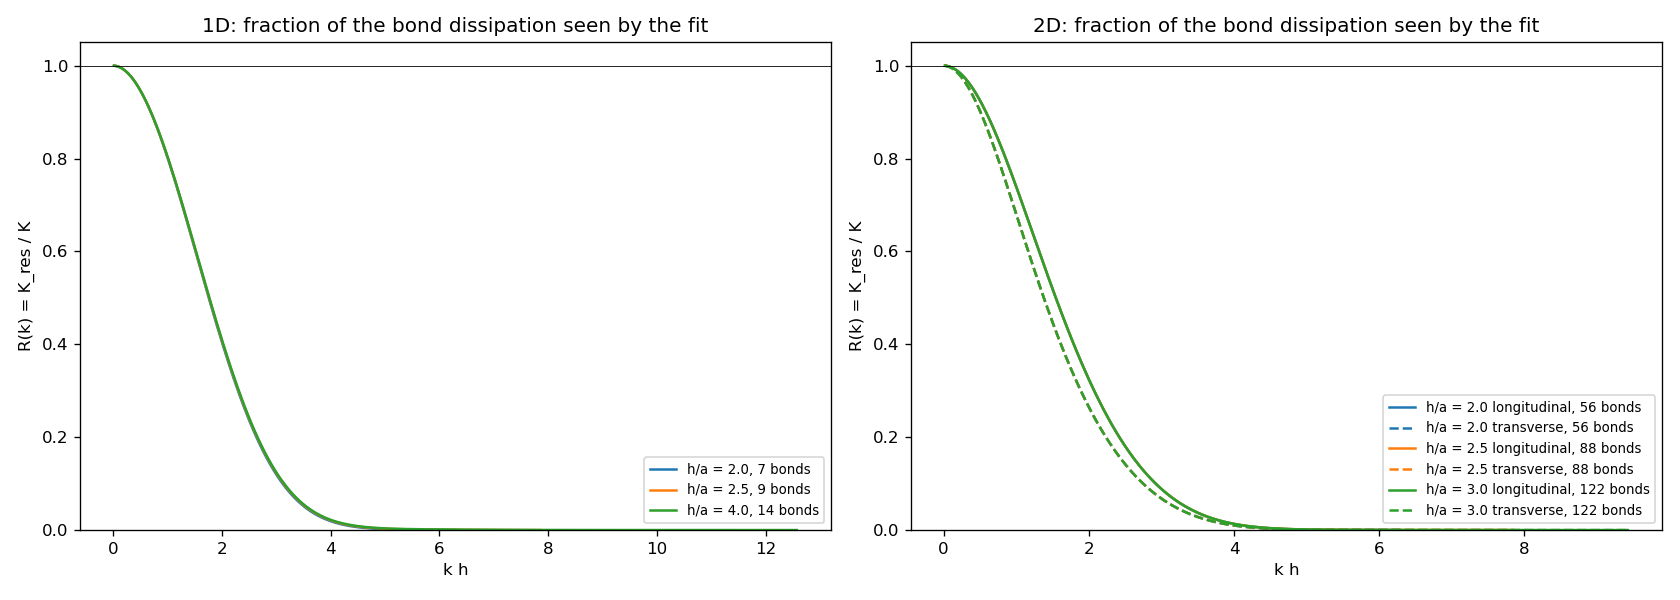
\includegraphics[width=\textwidth]{figs/stochrep_resolved_fraction.png}
\caption{The fraction $R(k)=K_{\rm res}(k)/K(k)$ of the bond dissipation seen by the fit,
versus $kh$, for several $h/a$.  Left: 1D.  Right: 2D, longitudinal (solid) and
transverse (dashed).  The curves for different $h/a$ coincide.}
\label{fig:Rk}
\end{figure}

\paragraph{Frozen lattice.}  \Fig{fig:stressonly}: the frozen lattice of
\texttt{stochrep.tex} ($h/a=2.5$, no Hamiltonian step), from zero momenta, with
the stress move only.  Each mode follows $1-e^{-2\Gamma_{\rm res}t}$.  The modes with
$kh\lesssim1$ thermalize as with both moves; those beyond $ka/\pi\simeq0.5$ have barely
moved by the end of the run.  The kinetic energy reaches $0.22$ of its
equilibrium value, against $0.99$ with both moves.

\begin{figure}[t]
\centering
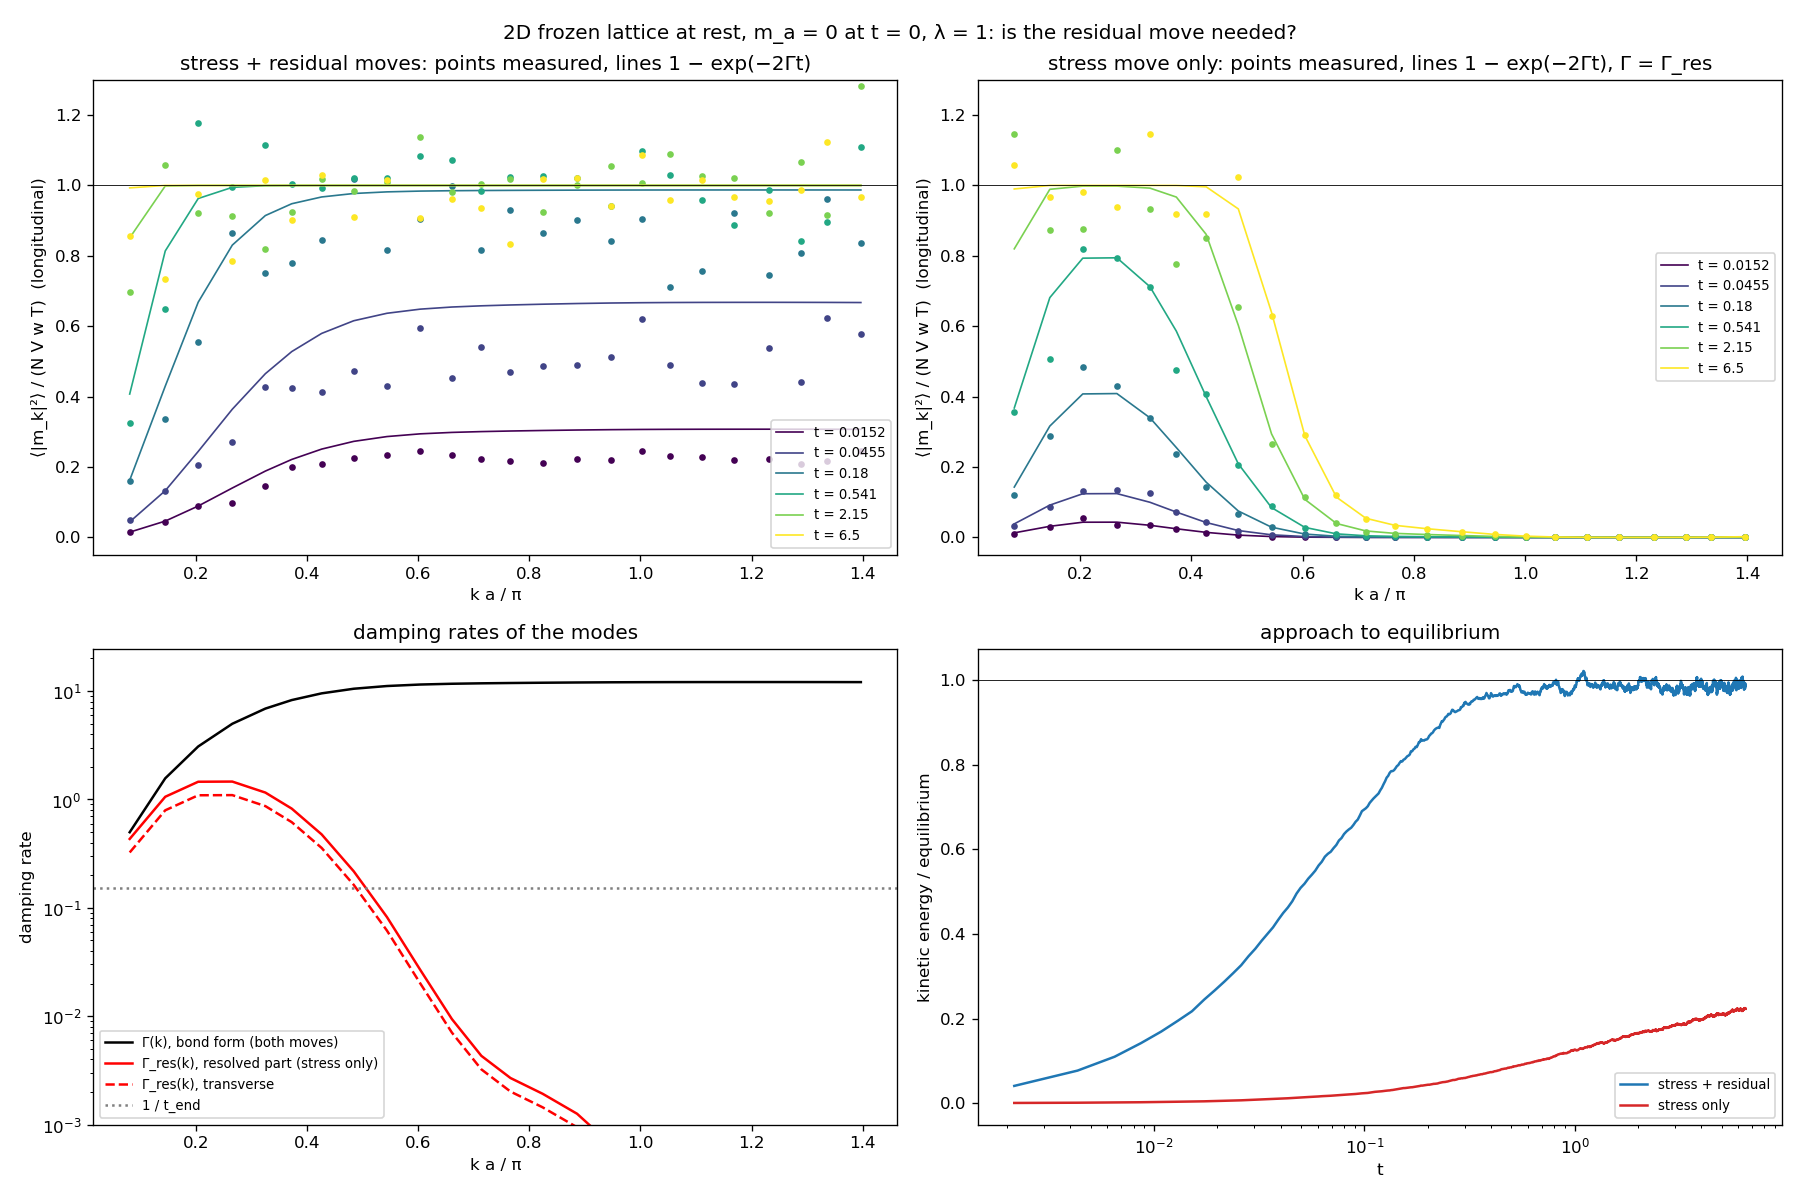
\includegraphics[width=\textwidth]{figs/stochrep_stressonly_2d.png}
\caption{2D frozen lattice ($h/a=2.5$) from zero momenta.  Top: the spectrum at
several times with both moves (left) and with the stress move only (right);
points measured, lines $1-e^{-2\Gamma t}$ with $\Gamma$ and $\Gamma_{\rm res}$.  Bottom
left: the two rates.  Bottom right: the kinetic energy.}
\label{fig:stressonly}
\end{figure}

\paragraph{With the Hamiltonian step.}  On a frozen lattice the unresolved modes
merely stay cold.  With the Hamiltonian step on they are driven by the ideal SPH
force, and nothing removes what it puts in.  \Fig{fig:hamiltonian} and
\Fig{fig:hamreal}: $h/a=2$, per-bond vote, plain map, to $t=15$.
\begin{itemize}
\item \emph{Stress and residual moves, $\lambda=1$.}  The spectrum is flat out to
  $kh\simeq9$ and the kinetic energy settles at its equilibrium value.  $H$ drops
  once by about $0.3\%$, as thermal energy moves into particle-scale fluctuations
  that the smoothed $H$ does not count.  It is then constant until $t\simeq8$, and
  afterwards creeps up by up to $0.1\%$ by $t=15$; $\sum_ae_a$ stays within
  $10^{-3}$.
\item \emph{Stress move and deterministic residual, $\lambda=\infty$.}  The lattice
  modes stay cold, the spectrum follows $T_{\rm eff}(k)$, and $H$ and $\sum_ae_a$
  are constant to about $10^{-4}$.
\item \emph{Stress move only.}  The modes with $kh\lesssim3$ look right, but the
  lattice modes are heated by the Hamiltonian step and not damped.  After
  $t\simeq6$ the kinetic energy grows exponentially, by about a factor $e$ per
  $3.5$ time units, and reaches 4 to 7 times its equilibrium value at $t=15$ in
  all four realizations; $\sum_ae_a$ grows with it, and the acceptance falls.
\end{itemize}
The same happens at $h/a=2.5$ (one realization).

In all three variants the particles drift away from the lattice.  Their rms
displacement reaches about one lattice spacing by $t=15$, mostly by collective
motion.  The local disorder reaches $0.18$--$0.27\,a$ with $\lambda=1$ or the stress
move alone, and $0.11$--$0.15\,a$ with $\lambda=\infty$.

\paragraph{Conclusion.}  The residual move is needed: it is what keeps the
lattice modes under control once the particles move.  For the modes with
$kh\ll1$ the stress move alone gives the right fluctuations, and the residual
can be cold ($\lambda>1$) or deterministic ($\lambda=\infty$) if the lattice modes need
not fluctuate.  The stress-only variant is dropped from here on.

\begin{figure}[t]
\centering
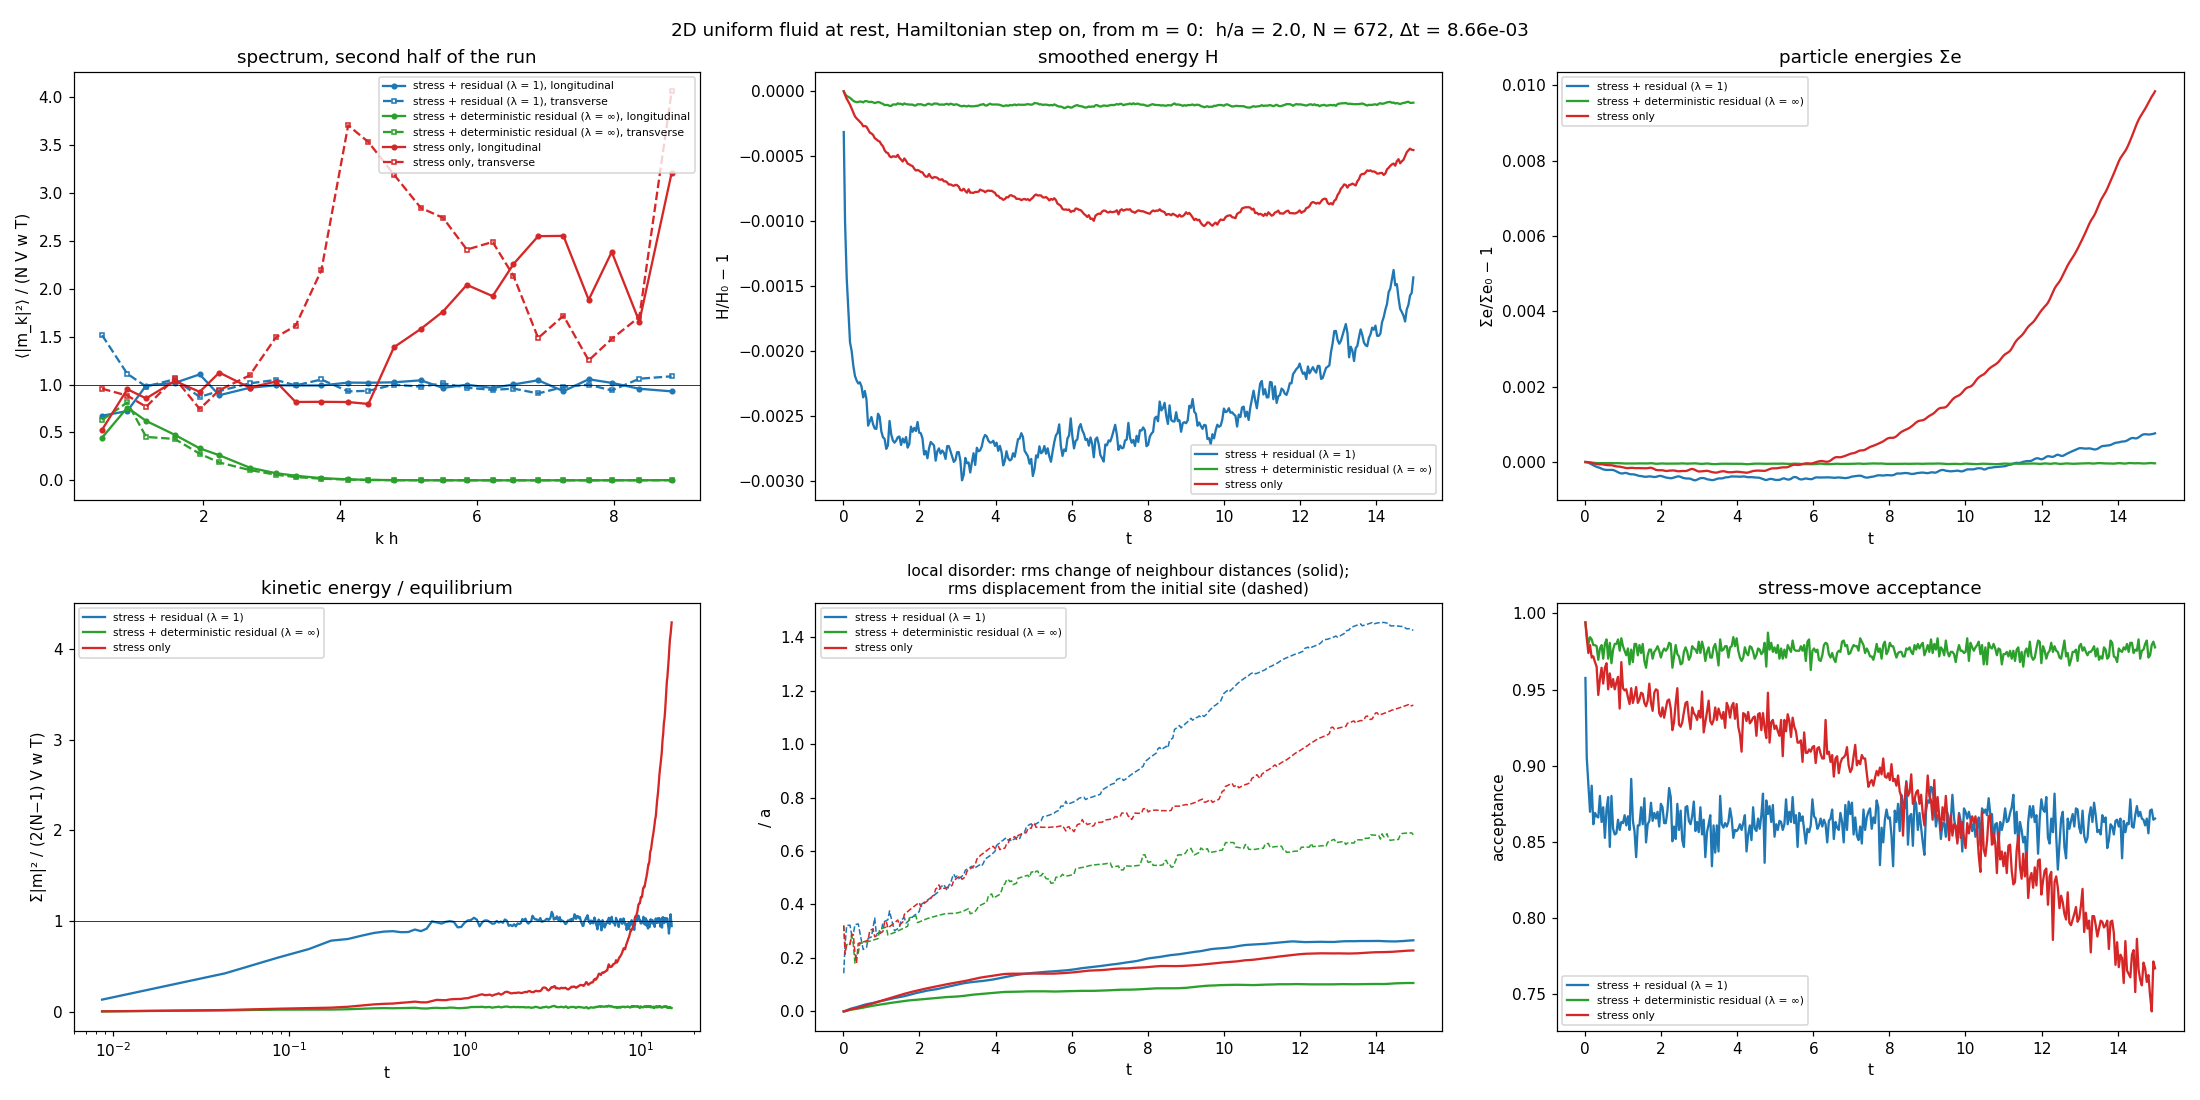
\includegraphics[width=\textwidth]{figs/stochrep_hamiltonian_ha2.0_t15.png}
\caption{$h/a=2$, per-bond vote, plain map, one realization of each variant, to
$t=15$.  Top: the spectrum over the second half of the run, the smoothed energy
$H$, and the particle energies $\sum_ae_a$.  Bottom: the kinetic energy; the local
disorder (solid) and the rms displacement (dashed); the acceptance of the
stress move.}
\label{fig:hamiltonian}
\end{figure}

\begin{figure}[t]
\centering
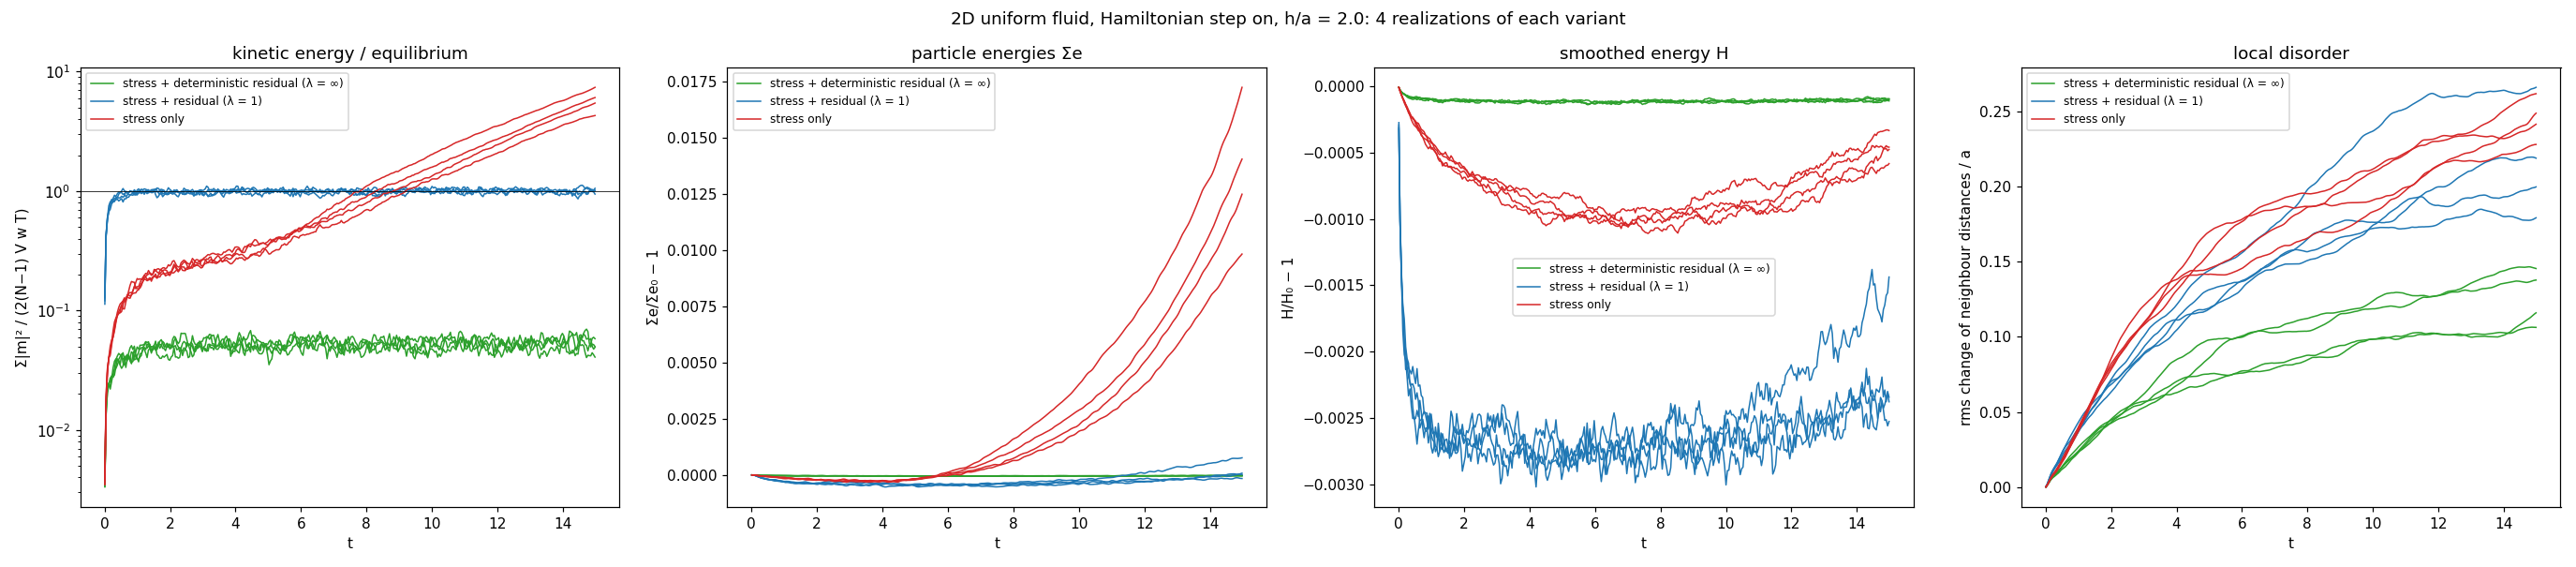
\includegraphics[width=\textwidth]{figs/stochrep_hamiltonian_real_ha2.0_t15.png}
\caption{As \Fig{fig:hamiltonian}, four realizations of each variant: kinetic
energy, particle energies, smoothed energy and local disorder.}
\label{fig:hamreal}
\end{figure}

%=============================================================================
\section{Longer runs: a slow heating}
\label{sec:t30}

\Fig{fig:t30}: the same setup to $t=30$, $\lambda=1$ and $\lambda=\infty$, four
realizations each, per-bond vote, plain map.
\begin{itemize}
\item \emph{$\lambda=\infty$}: the kinetic energy, $H$, $\sum_ae_a$ and the local
  disorder all level off; $H$ and $\sum_ae_a$ change by less than $10^{-4}$.
\item \emph{$\lambda=1$}: the kinetic energy stays at its equilibrium value, but
  after $t\simeq8$ both $\sum_ae_a$ and $H$ rise, faster and faster, in all four
  runs: $\sum_ae_a$ by $0.24$--$0.45\%$ and $H$ by $0.3$--$0.5\%$ from its minimum, by
  $t=30$.  The fluid heats slowly.  The local disorder keeps growing, to
  $0.25$--$0.35\,a$.
\end{itemize}

\begin{figure}[t]
\centering
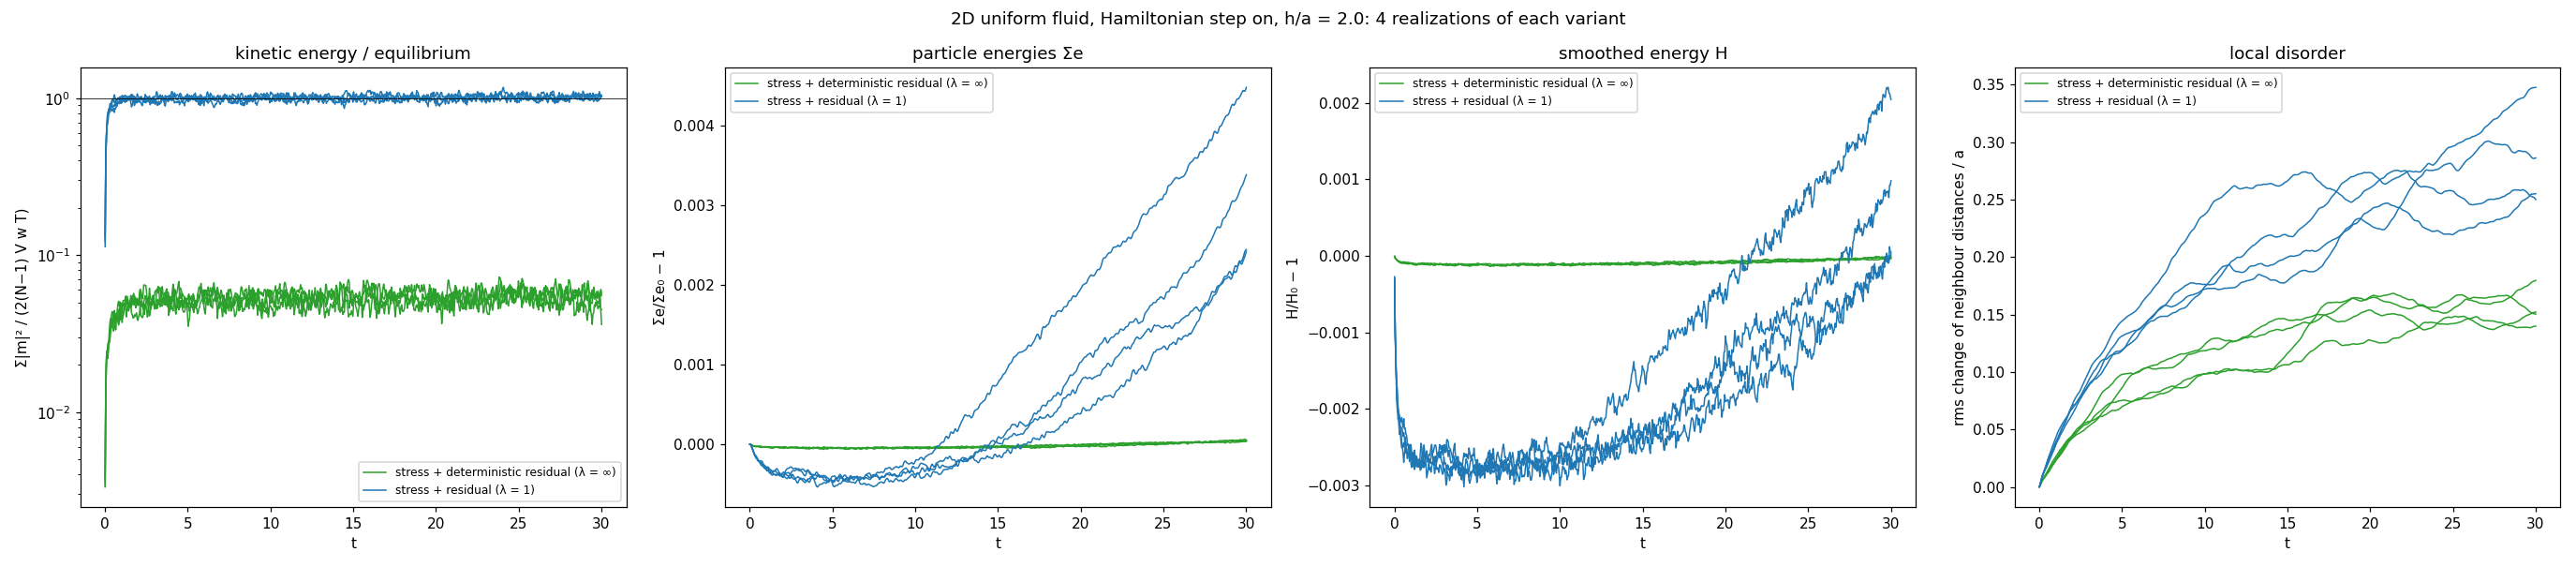
\includegraphics[width=\textwidth]{figs/stochrep_hamiltonian_real_ha2.0_t30.png}
\caption{$h/a=2$, per-bond vote, plain map, to $t=30$, four realizations of
$\lambda=1$ and $\lambda=\infty$: kinetic energy, particle energies, smoothed energy and
local disorder.}
\label{fig:t30}
\end{figure}

%=============================================================================
\section{The single vote}
\label{sec:star}

\Fig{fig:star}: as \Sect{sec:t30} with a single vote of the star in place of
the per-bond vote.  The residual move is accepted about $0.88$ of the time
instead of about $0.5$, so the lattice modes are damped faster.  The heating is
about halved and starts later: at $t=30$, $\sum_ae_a$ has changed by $-0.05$ to
$+0.13\%$, and three of the four runs are close to flat.  One run turns upward
from $t\simeq20$; it is also the run with the largest local disorder, $0.31\,a$.
$\lambda=\infty$ is again flat.

\begin{figure}[t]
\centering
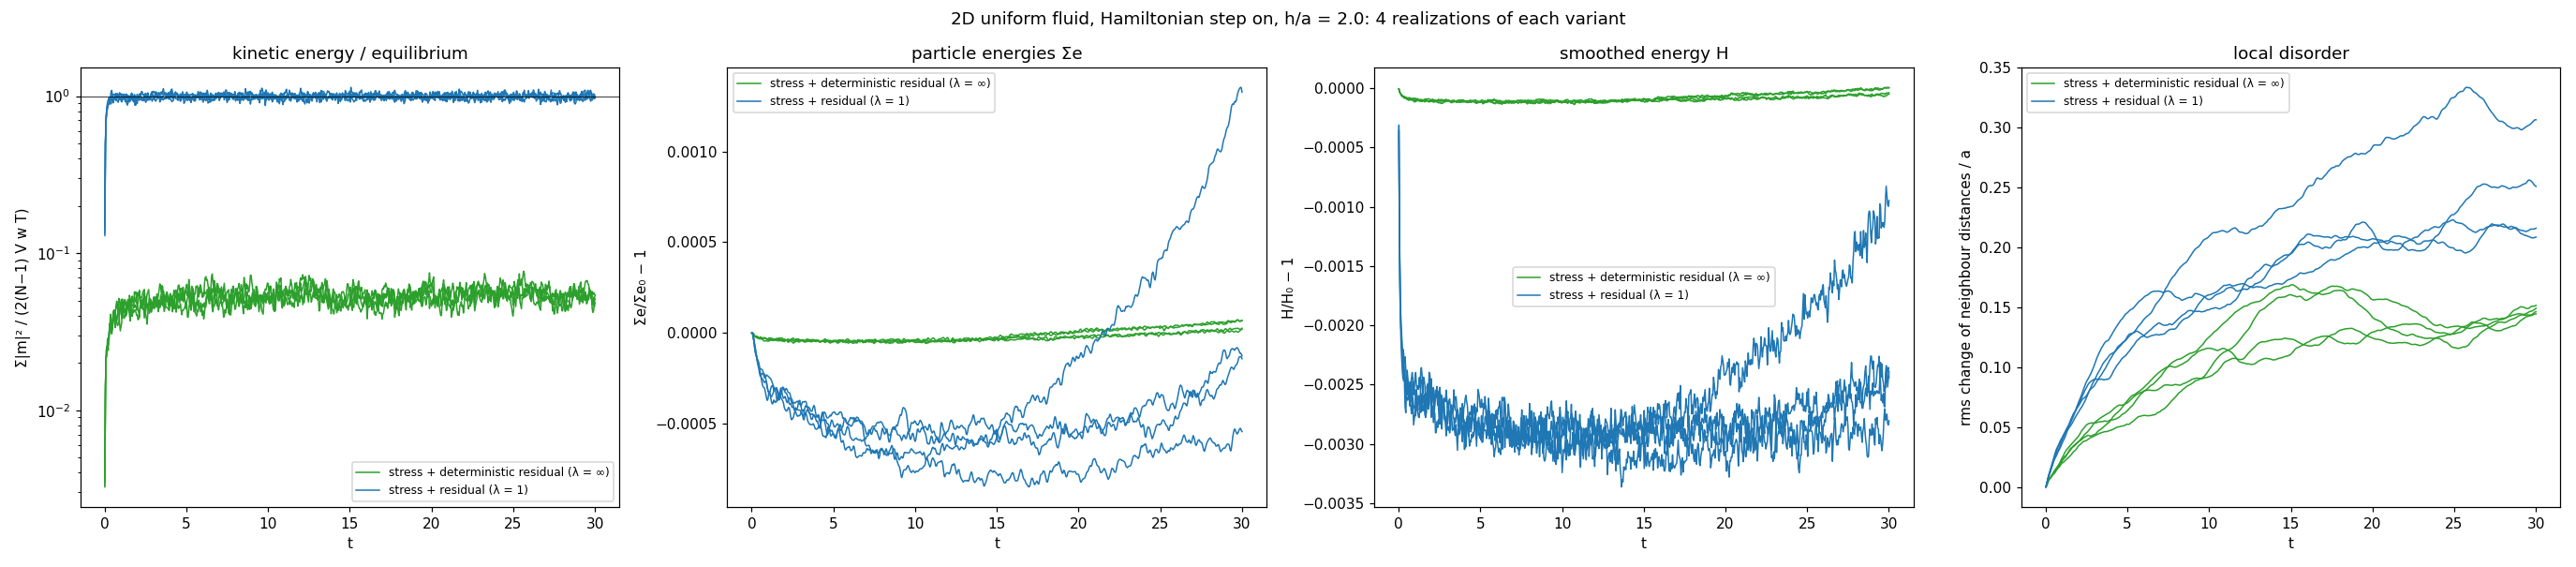
\includegraphics[width=\textwidth]{figs/stochrep_hamiltonian_real_ha2.0_t30_star.png}
\caption{As \Fig{fig:t30}, with the single vote of the star.}
\label{fig:star}
\end{figure}

%=============================================================================
\section{Where the energy changes}
\label{sec:split}

To locate the heating, each time step is split: the change of $H$ and of
$\sum_ae_a$ in the two stochastic half steps, and in the leapfrog, accumulated
over the run.  \Fig{fig:split}: $\lambda=1$, single vote, at $\Delta t$ and $\Delta t/2$, four
realizations each.
\begin{itemize}
\item \emph{The leapfrog conserves $H$ to about $10^{-7}$,} at both time steps.
  The integrator is not the source.
\item \emph{All the change of $H$ comes from the stochastic half steps:} the
  initial drop, the plateau, and the late rise.  The late rise is smaller at
  $\Delta t/2$, where all four runs stay within $-2.5$ to $-2.9\times10^{-3}$.
\item \emph{The stochastic half steps lose $\sum_ae_a$ at a steady rate,} the same
  in every run: about $-4\times10^{-5}$ per unit time.  Within a step each $e_a$
  is fixed at the frozen volume; afterwards $s_a$ has changed by a random amount
  and the re-smoothing gives new volumes and energies.  The first-order effect
  averages to zero; the second-order one does not, and accumulates linearly.
  It is an It\^o-type term of the change of representation.
\item \emph{The leapfrog raises $\sum_ae_a$ slowly}, by $0.07$--$0.12\%$ at $t=30$.
  Since it conserves $H$, this is the gap $\sum_ae_a-H$ changing as the
  arrangement of the particles disorders.
\end{itemize}

\begin{figure}[t]
\centering
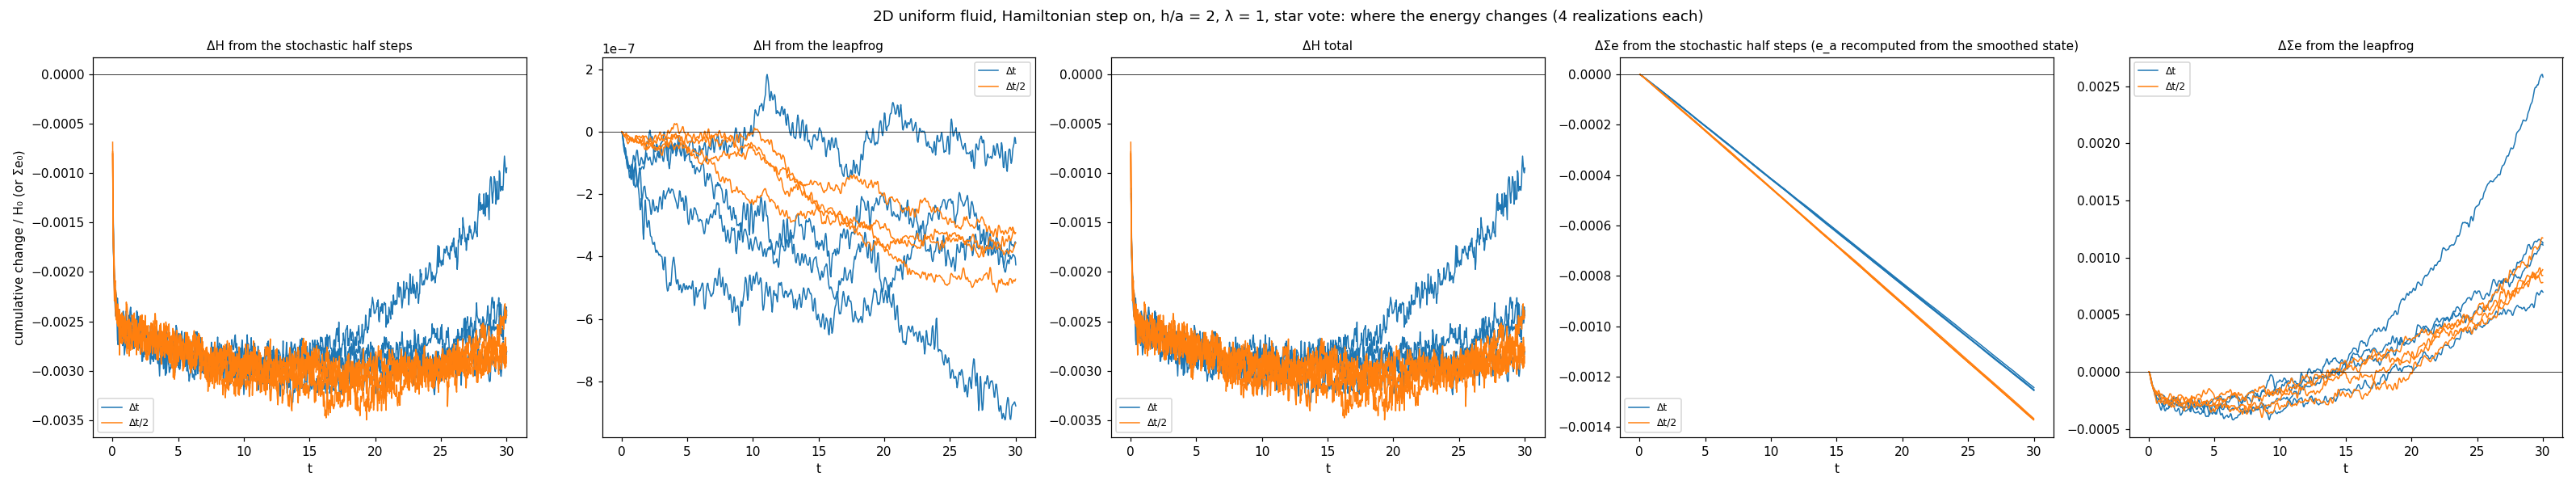
\includegraphics[width=\textwidth]{figs/stochrep_hamiltonian_split_dt0.5.png}
\caption{$h/a=2$, $\lambda=1$, single vote, plain map, at $\Delta t$ and $\Delta t/2$: cumulative
changes of $H$ from the stochastic half steps, from the leapfrog, and in total,
and of $\sum_ae_a$ from the stochastic half steps and from the leapfrog.}
\label{fig:split}
\end{figure}

%=============================================================================
\section{The gradient-corrected change of representation}
\label{sec:grad}

The stochastic step changes representation twice per time step, between the
smoothed variables of the leapfrog and the particle representation.  The
gradient-corrected map, which removed most of the energy drift of the
deterministic step (\texttt{changerep.tex}), is now used here too: the gradient
energy $g_a$ is frozen during the sweeps, so the sweeps and their equilibrium
are unchanged, and the back map refits it.  \Fig{fig:gradsplit} and
\Fig{fig:grad}: $\lambda=1$, single vote, $\Delta t$, four realizations.
\begin{itemize}
\item The kinetic energy stays at its equilibrium value.
\item $\sum_ae_a$ stays within $\pm5\times10^{-4}$ (plain map: $-5\times10^{-4}$ to
  $+1.3\times10^{-3}$).
\item $H$, after the one-time drop of about $0.25\%$, stays within $-2.9$ to
  $-1.8\times10^{-3}$, with a gentle late rise.
\item The local disorder levels off at $0.18$--$0.28\,a$.
\item The steady loss of $\sum_ae_a$ in the stochastic steps is unchanged: it comes
  from the random change of $s_a$, not from the gradient energy.  The one-time
  drop of $H$ is also unchanged: the correction captures the smooth part of the
  momentum field, not its thermal particle-scale fluctuations.
\end{itemize}
The remaining drift is small and smooth; a global thermostat can remove it if
needed.

\begin{figure}[t]
\centering
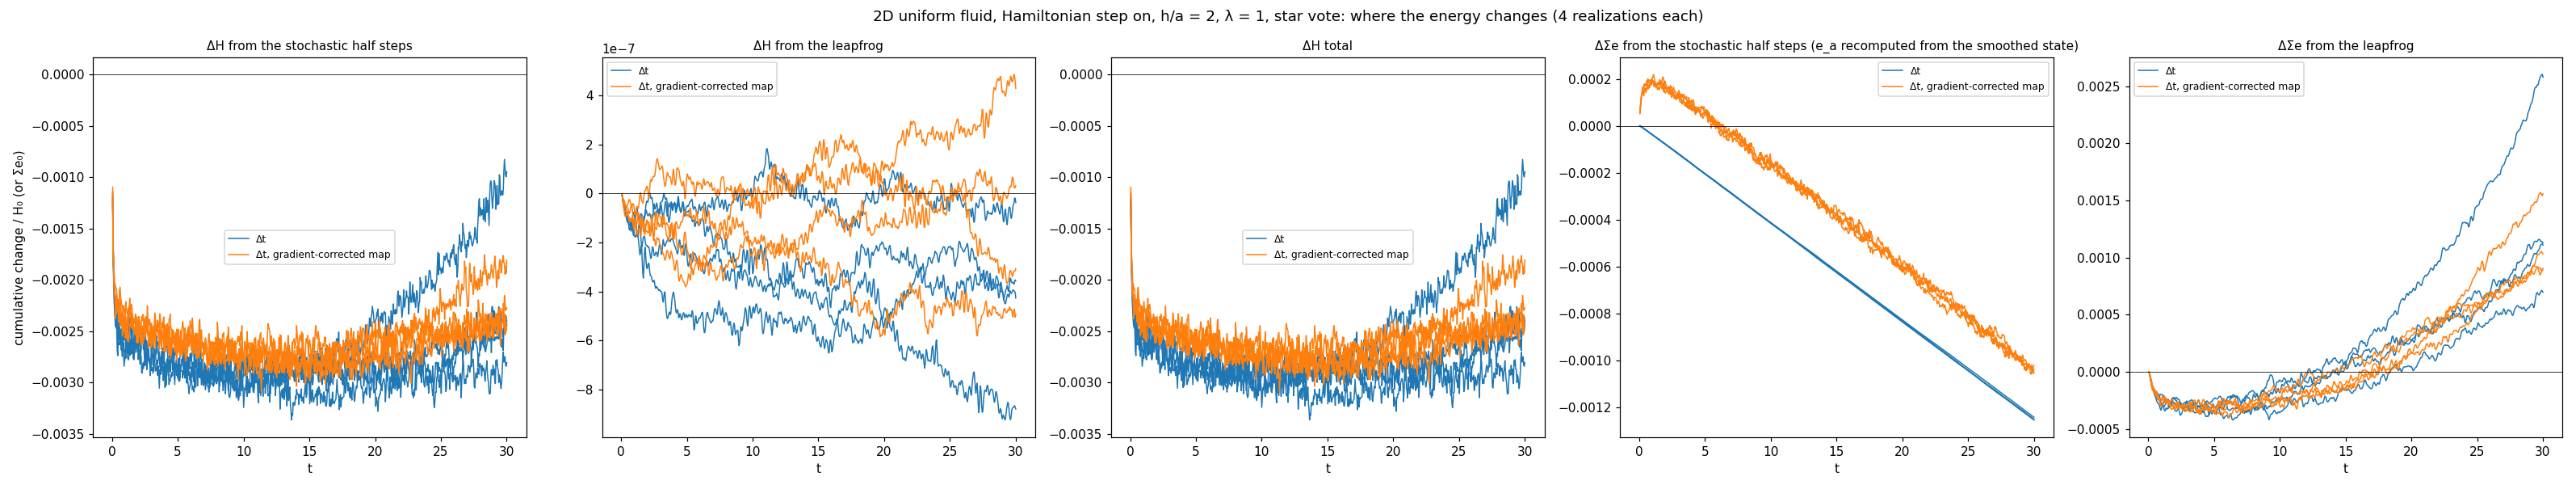
\includegraphics[width=\textwidth]{figs/stochrep_hamiltonian_split_grad.png}
\caption{As \Fig{fig:split}, plain map and gradient-corrected map at $\Delta t$.}
\label{fig:gradsplit}
\end{figure}

\begin{figure}[t]
\centering
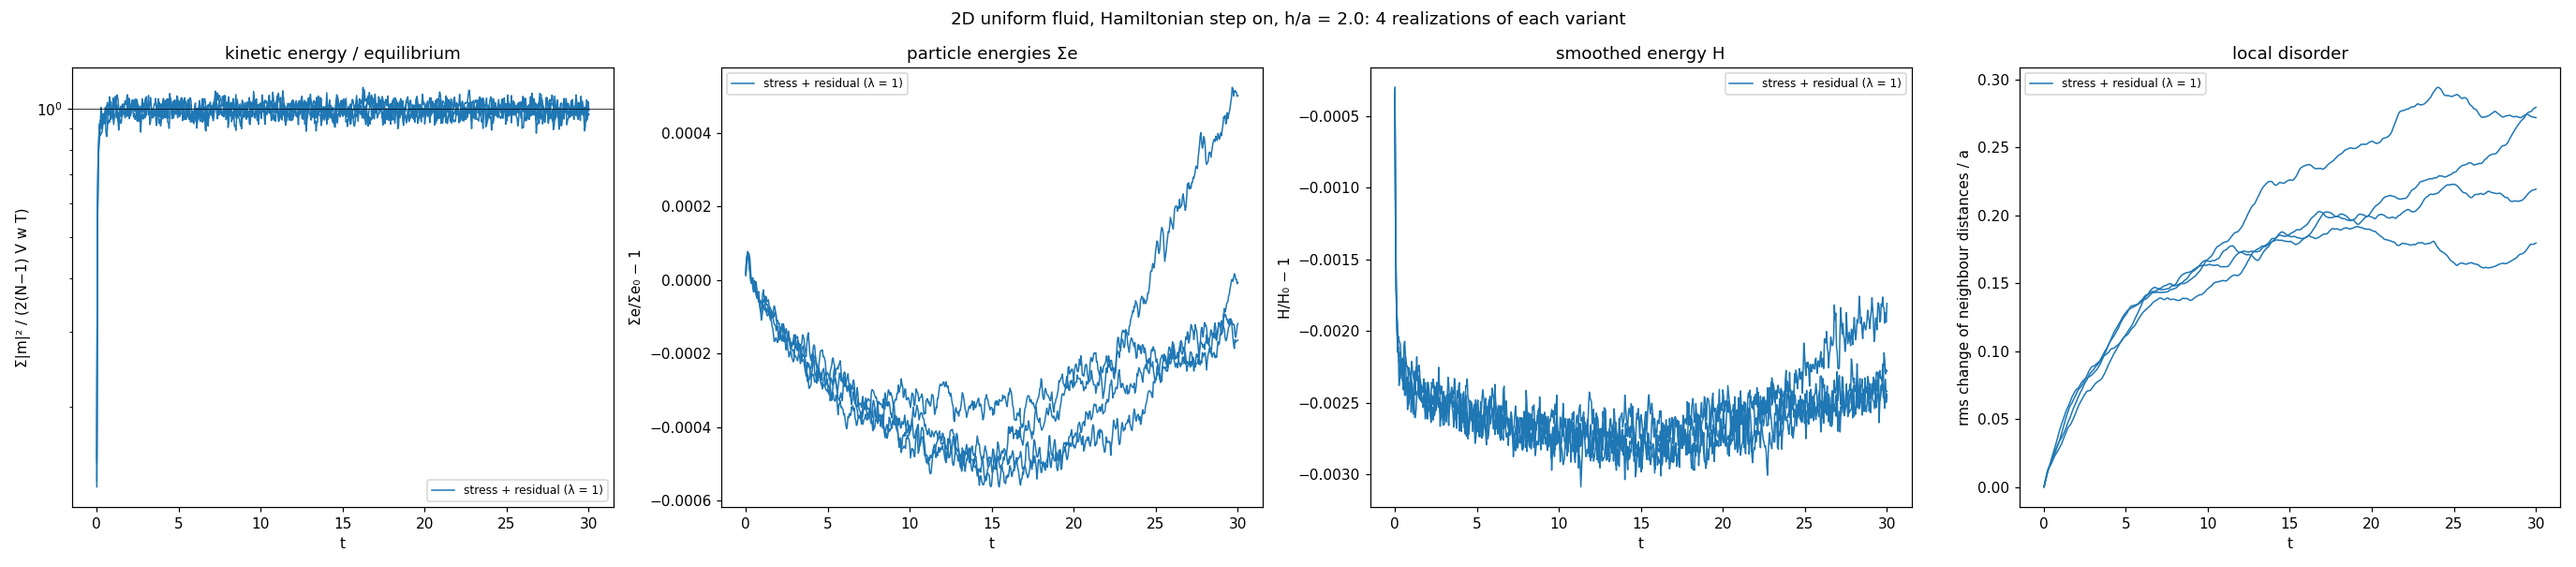
\includegraphics[width=\textwidth]{figs/stochrep_hamiltonian_real_ha2.0_t30_star_grad.png}
\caption{$h/a=2$, $\lambda=1$, single vote, gradient-corrected map, to $t=30$, four
realizations: kinetic energy, particle energies, smoothed energy and local
disorder.}
\label{fig:grad}
\end{figure}

%=============================================================================
\section{Long runs}
\label{sec:long}

Runs to $t=100$, four realizations each, all at rest, to see how the long-time
behaviour depends on the parameters.  The reference is $h/a=2$, $\lambda=1$, single
vote, gradient-corrected map, $\Delta t=8.66\times10^{-3}$; each run changes one thing:
\begin{center}
\begin{tabular}{ll}
\hline
reference & also $\lambda=\infty$ \\
time step & $\Delta t/2$ \\
vote & per bond \\
map & plain (no gradient correction) \\
viscosity & $\eta/s=0.1$ \\
fluctuations & $S=10^5$: $s_a=54$, thermal velocity $0.14$ \\
spacing & $h/a=2.5$ \\
\hline
\end{tabular}
\end{center}
Each set has four realizations; \Fig{fig:long} shows them as bands, and
\Fig{fig:S1e5} the set with larger fluctuations, which behaves differently.
\begin{center}
\begin{tabular}{lcccc}
\hline
set & kinetic energy & $\Delta\sum_ae_a/\sum_ae_a$ & $\Delta H/H$ & local disorder \\ \hline
reference & $1.05$ & $+1.2\%$ & $+0.9\%$ & $0.27\,a$ \\
$\lambda=\infty$ & $0.05$ & $+0.09\%$ & $+0.09\%$ & $0.19\,a$ \\
$\Delta t/2$ & $1.03$ & $+1.0\%$ & $+0.8\%$ & $0.30\,a$ \\
per-bond vote & $1.10$ & $+4.1\%$ & $+3.8\%$ & $0.31\,a$ \\
plain map & $1.00$ & $+1.45\%$ & $+1.2\%$ & $0.30\,a$ \\
$\eta/s=0.1$ & $1.09$ & $+4.1\%$ & $+3.9\%$ & $0.31\,a$ \\
$h/a=2.5$ & $1.00$ & $+0.7\%$ & $+0.3\%$ & $0.51\,a$ \\
$S=10^5$ & $4\times10^4$ & $\times50$ & $\times32$ & $3.4\,a$ \\
\hline
\end{tabular}
\end{center}
(Values at $t=100$, averaged over the realizations; the kinetic energy relative
to its equilibrium value at the initial temperature.)

\paragraph{Slow heating everywhere.}  In every set with $\lambda=1$ the energies
rise, slowly at first and faster later.  The local disorder levels off at
$0.27$--$0.31\,a$ for $h/a=2$ after $t\simeq30$, but the heating does not stop.

\paragraph{What it depends on.}
\begin{itemize}
\item \emph{Viscosity}: halving $\eta/s$ makes the heating about $3.5$ times faster.
\item \emph{Vote}: the per-bond vote, which rejects more residual moves and
  so damps the lattice modes more slowly, heats as fast as $\eta/s=0.1$.
\item \emph{Time step}: halving $\Delta t$ helps only a little ($-15\%$).
\item \emph{Change of representation}: the gradient-corrected map heats about
  $20\%$ less than the plain map.
\item \emph{Spacing}: $h/a=2.5$ heats less, although its lattice disorders more.
\item \emph{$\lambda=\infty$}: the lattice modes are cold and the heating is ten times
  slower.
\item \emph{Fluctuations}: with $S=10^5$ (entropy per particle $54$, thermal
  velocity $0.14$, three times larger) the lattice melts within $t\simeq40$, the
  local disorder passing one lattice spacing, and then the energies grow
  exponentially, by a factor $e$ in about $4.5$ time units, to fifty times their
  initial value by $t=100$.  This is an instability, not a drift.
\end{itemize}

\paragraph{Interpretation (to be tested).}  The heating grows with the size of
the thermal fluctuations and falls with the damping of the lattice modes
(viscosity, acceptance, $\lambda$).  This points to the lattice modes: the ideal
step on a thermally agitated, disordering arrangement feeds them, and the
viscous step removes it.  When the fluctuations are too large compared with
the damping, the lattice melts and the feeding wins.  The energy split
(\Sect{sec:split}) places the change of $H$ in the stochastic step; for the
unstable set it is being measured.  A criterion for stability, in terms of the
thermal velocity, the viscosity and $h$, is the most important open question
for production runs.

\begin{figure}[t]
\centering
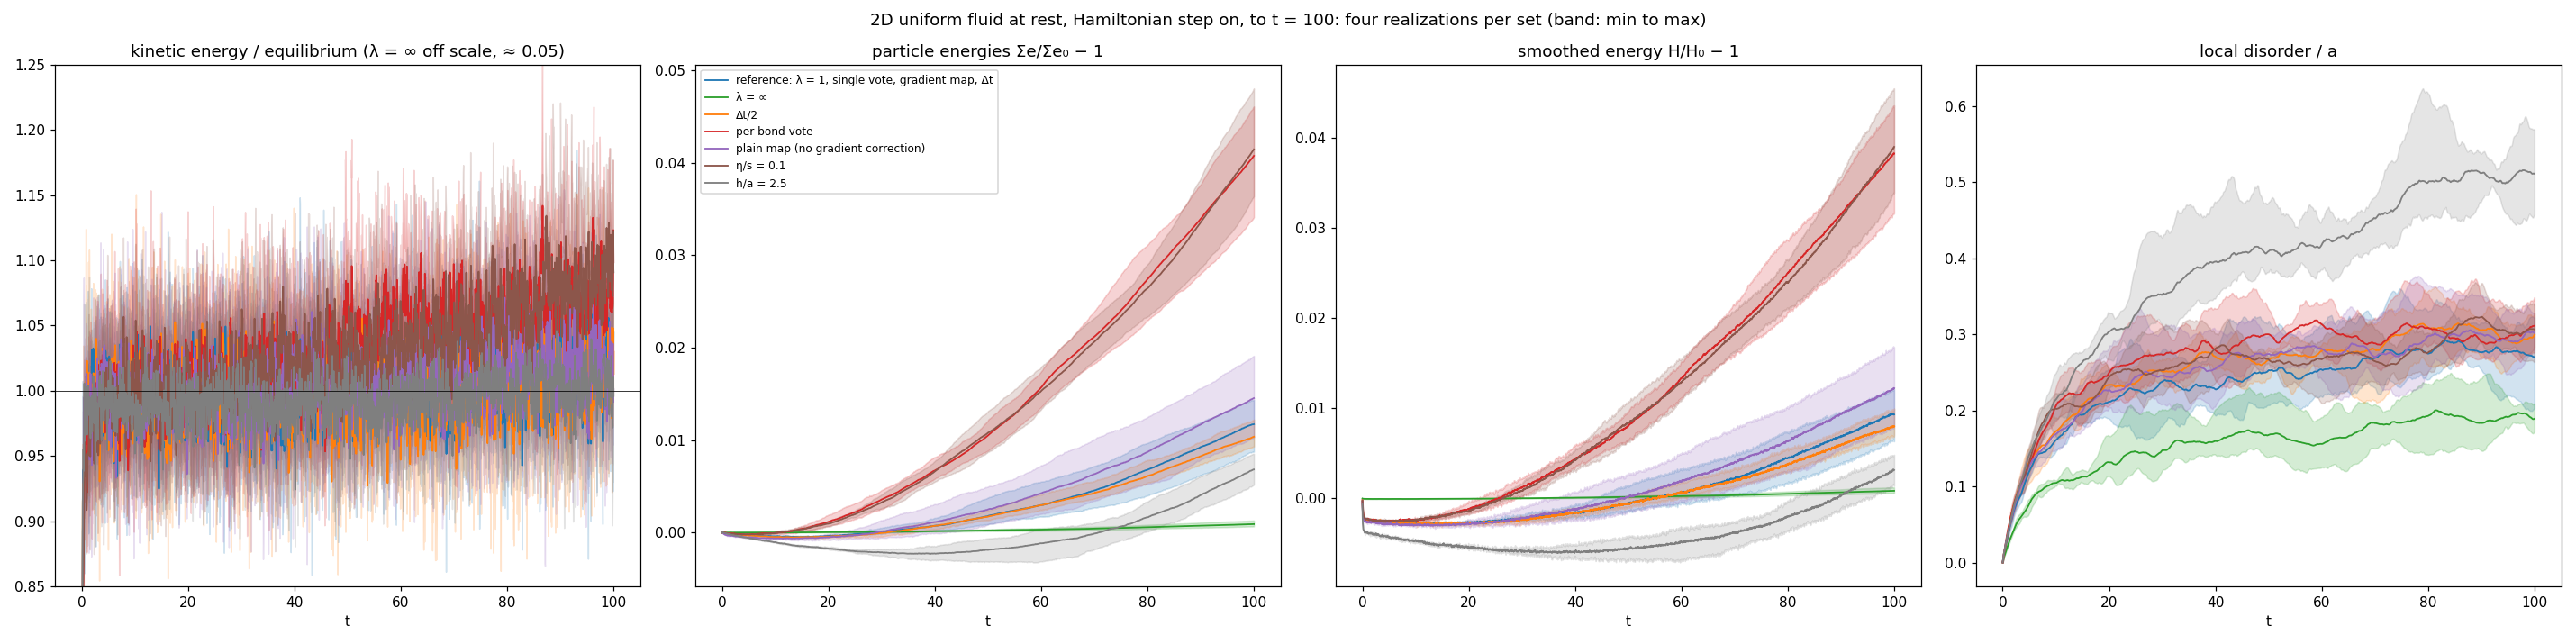
\includegraphics[width=\textwidth]{figs/stochrep_longruns.png}
\caption{Runs to $t=100$, four realizations per set (band: minimum to maximum,
line: mean).  Kinetic energy, particle energies, smoothed energy and local
disorder.  The set with $S=10^5$ is shown separately in \Fig{fig:S1e5}.}
\label{fig:long}
\end{figure}

\begin{figure}[t]
\centering
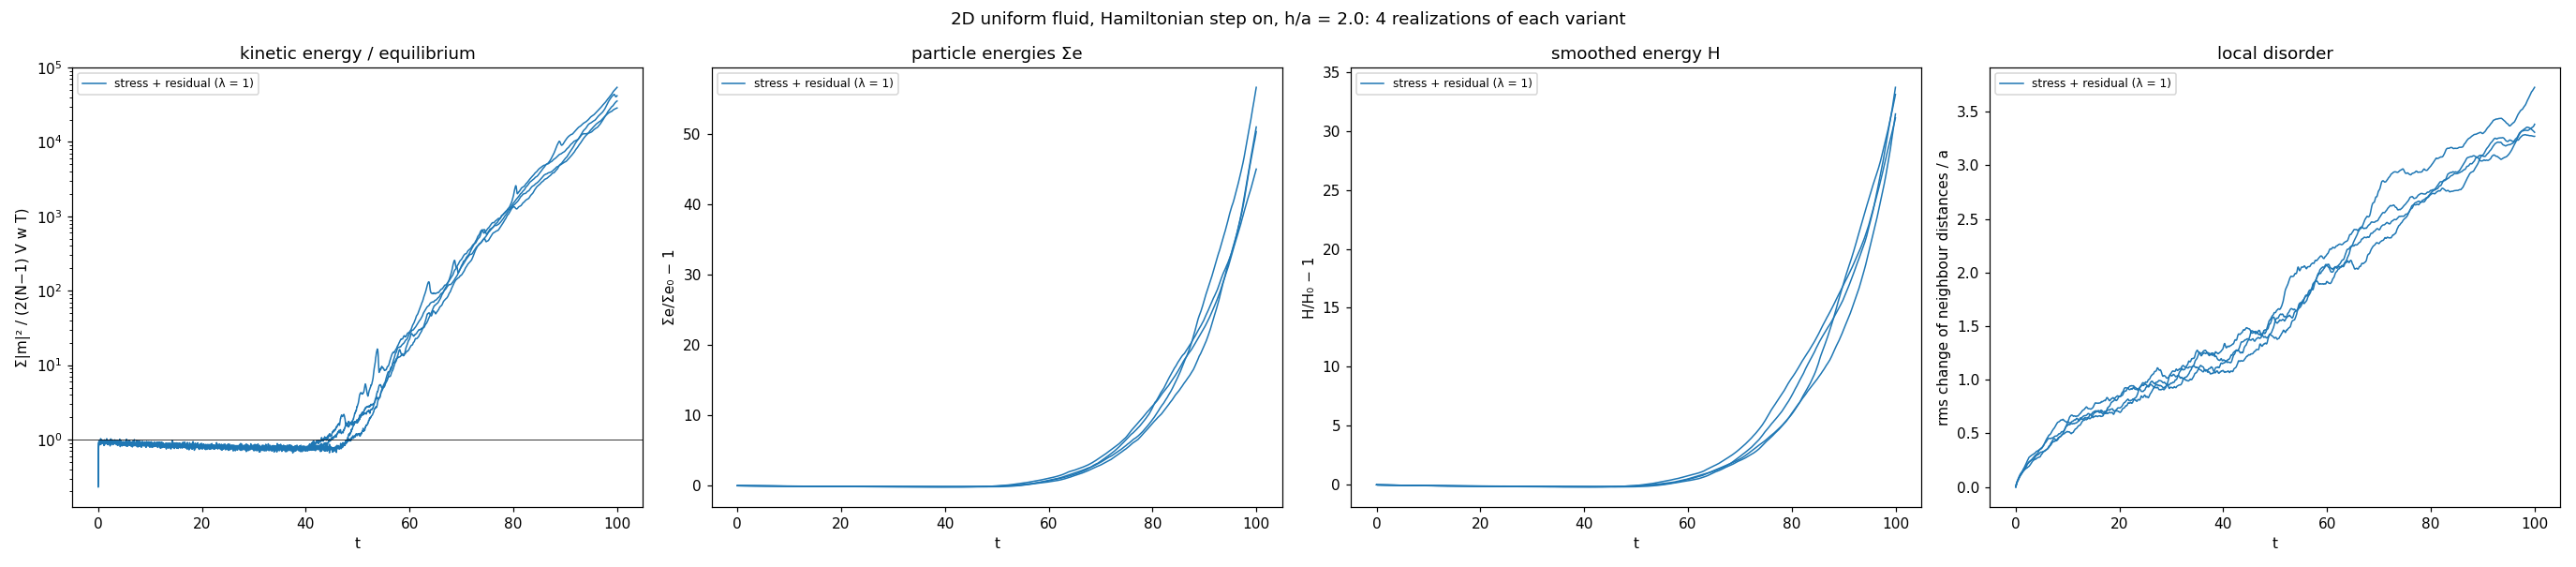
\includegraphics[width=\textwidth]{figs/stochrep_hamiltonian_real_ha2.0_t100_star_grad_S100000.0.png}
\caption{$S=10^5$ (entropy per particle $54$, thermal velocity $0.14$): four
realizations.  The lattice melts by $t\simeq40$; the energies then grow
exponentially.}
\label{fig:S1e5}
\end{figure}

%=============================================================================
\section{Summary}
\label{sec:summary}

\begin{itemize}
\item The residual move is needed once the particles move; without it the
  lattice modes run away.
\item With both moves, $\lambda=1$, the fluid thermalizes in about one time unit and
  stays at equilibrium, with a flat spectrum, out to $t=30$.
\item $H$ drops once by about $0.3\%$ as the particle-scale fluctuations fill in,
  then drifts slowly.  The drift comes from the stochastic step, not from the
  leapfrog; it is reduced by the single vote, by a smaller time step and by
  the gradient-corrected map.
\item With $\lambda=\infty$ the lattice modes stay cold and the energies are constant to
  $10^{-4}$ at $t=30$ and to $10^{-3}$ at $t=100$.
\item To $t=100$ every $\lambda=1$ set heats slowly, faster for smaller viscosity or a
  vote that rejects more.  With three times larger thermal velocities the lattice
  melts and the energies blow up: the scheme has a stability limit, set by the
  fluctuations against the damping, which must be found before production runs.
\end{itemize}

\end{document}
